\documentclass[aspectratio=169,notes]{beamer}
\usepackage{graphicx}
\usepackage{hyperref}
\usetheme{metropolis}
\title{Heat Injuries}
\institute{Engineers for Exploration, UC San Diego}
\logo{
\includegraphics[height=.65cm,keepaspectratio]{e4e_logo_350x136.png}}
\setbeamertemplate{caption}[numbered]
\begin{document}
\maketitle
\begin{frame}
    \centering
    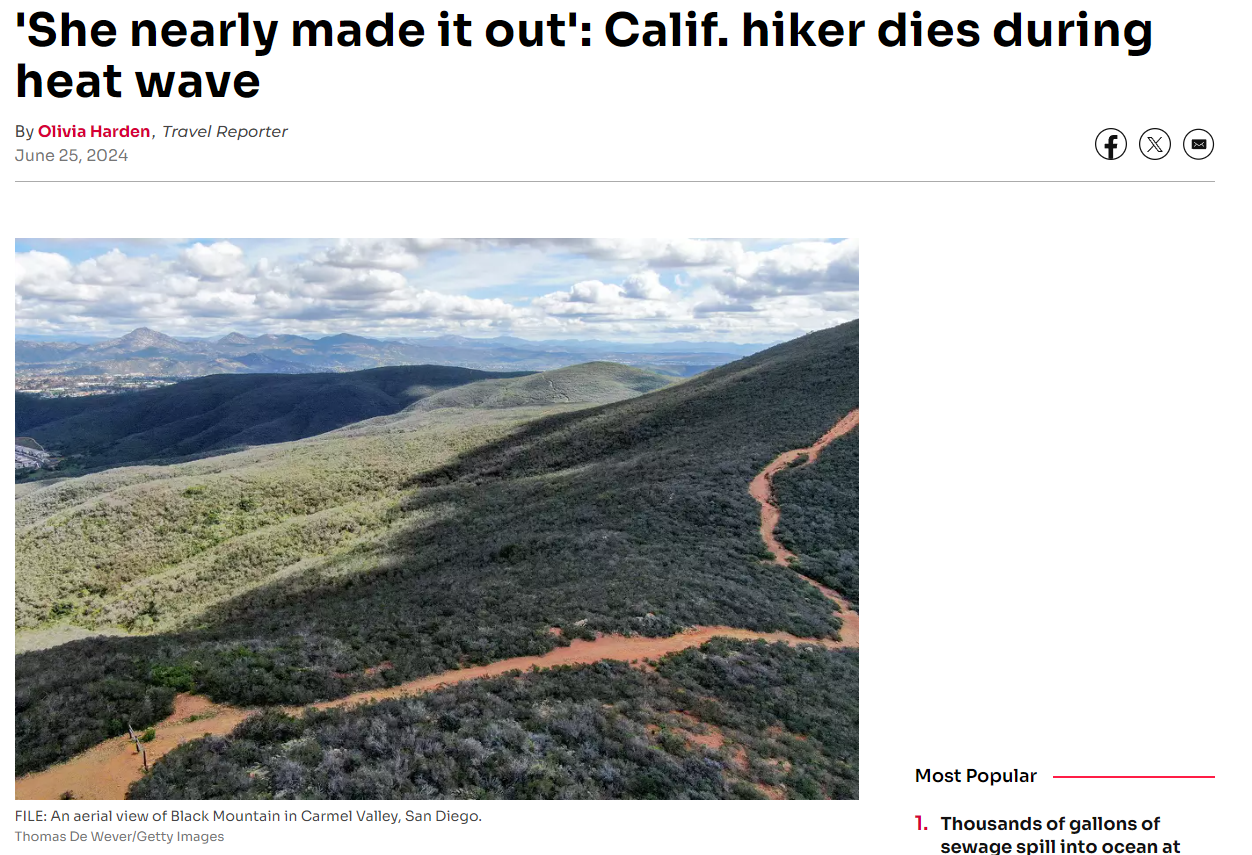
\includegraphics[width=0.8\textwidth, height=0.8\textheight, keepaspectratio]{2024-06-25-sfgate-california-hiker-dies-heat-wave.png}
\end{frame}
\begin{frame}{Statistics - Average}
    \begin{enumerate}
        \item Heat is the \#1 weather-releated killer in the United States ($\approx$ 123/yr)
        \item Greater than hurricanes ($\approx$ 108), floods ($\approx$ 75), and lightning strikes ($\approx$ 33)
        \item Even more than tornadoes ($\approx$ 109)
    \end{enumerate}
\end{frame}
\begin{frame}{Heat Stress is a Big Deal}
    \begin{itemize}
        \item Heat stress happens when your body loses its ability to self-regulate body temperature.
        \item Heat stress can lead to a range of heat-induced conditions (from least serious to most serious): heat rash, heat cramps, fainting, heat exhaustion, heat stroke.
        \item For outdoor workers, the sun is the biggest cause of heat stress. They are at a much higher risk of heat stress (for example, agricultural workers in the USA are at 20 times the risk than the national rate) 
    \end{itemize}
\end{frame}
\begin{frame}{Serious Outcomes of Heat Stress}
    \begin{itemize}
        \item Heat illness caused by heat stress can be a matter of life and death. Workers die from heat stroke every summer and every death is preventable.
        \item When heat stroke doesn't kill immediately, it can shut down major body organs causing acute heart, liver, kidney and muscle damage, nervous system problems, and blood disorders.
    \end{itemize}
\end{frame}
\begin{frame}
    \centering
    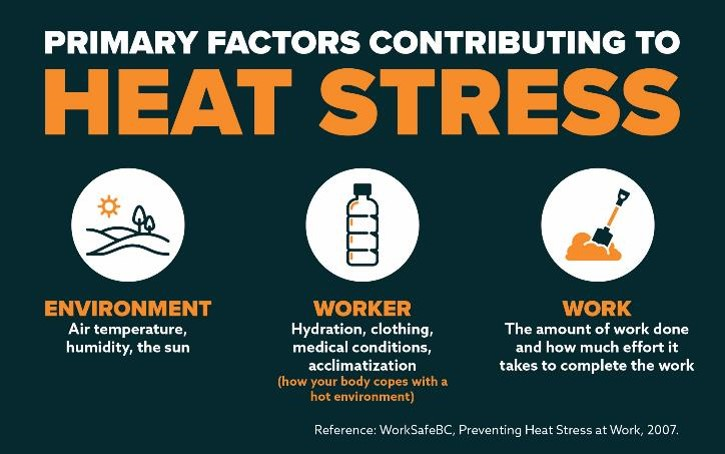
\includegraphics[width=0.8\textwidth, height=0.8\textheight, keepaspectratio]{primary_factors.jpg}
\end{frame}
\begin{frame}{Contributing Factors to Heat Stress}
    \begin{itemize}
        \item Previous heat injury
        \item Alcohol consumption
        \item Some dietary supplements
        \item Fatigue
        \item Skin trauma (sunburn)
    \end{itemize}
\end{frame}
\begin{frame}{An ounce of prevention is worth a pound of cure}
    \begin{itemize}
        \item Hydration is key
        \begin{itemize}
            \item Drink plenty of fluids
            \item Avoid caffeine, alcohol, sugary drinks, or very cold drinks
        \end{itemize}
        \item Access to cooling
        \begin{itemize}
            \item Passive cooling
            \begin{itemize}
                \item Shade
                \item Reflective clothing
            \end{itemize}
            \item Active cooling
            \begin{itemize}
                \item Ice vests
                \item Wetted clothing (low humidity environments)
                \item Water cooled garments
                \item Circulating air
            \end{itemize}
        \end{itemize}
    \end{itemize}
\end{frame}
\begin{frame}{An ounce of prevention is worth a pound of cure (cont.)}
    Be aware of conditions

    \centering
    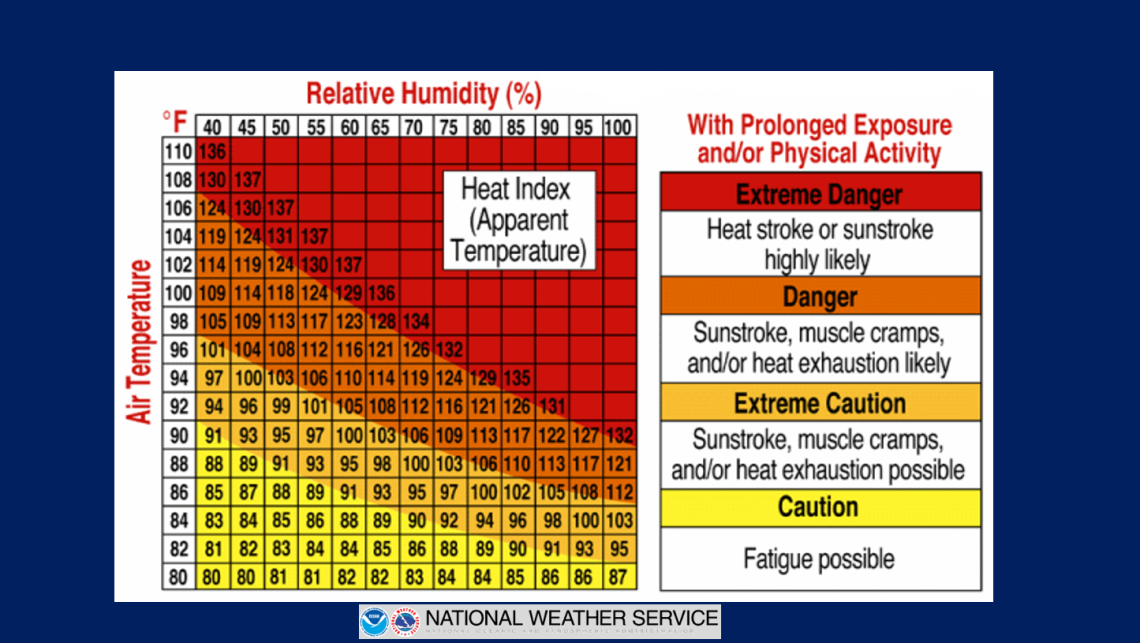
\includegraphics[width=0.6\textwidth,height=0.5\textheight,keepaspectratio]{Heat Index NWS.png}
\end{frame}
\end{document}
